I recommender system (RS) sono algoritmi mirati a generare consigli significativi a un insieme di utenti per articoli o prodotti che potrebbero interessarli \cite{recsys-definition}. La definizione di oggetto è generica e include ad esempio film da guardare, libri da leggere, prodotti da comprare, punti di interesse, etc. 
Quando gli utenti interagiscono con il sistema di raccomandazione generano dei feedback. Questi feedback possono essere di due tipi: espliciti o impliciti. I feedback espliciti sono valori numerici che un utente assegna ad un prodotto; i feedback impliciti riflettono indirettamente le opinioni di un utente osservando la cronologia degli acquisti, i link aperti, gli elementi visualizzati, etc.
Basandosi sui feedback passati, i sistemi di raccomandazione imparano un modello per prevedere quanto un utente può essere interessato a nuovi oggetti. Questi oggetti sono poi ordinati in base alla pertinenza prevista per l'utente. In ultimo, gli oggetti con il rank più alto vengono suggeriti all'utente. La relazione tra utenti e oggetti è rappresentata con una matrice $R_M$ in cui sono memorizzati i rating passati degli utenti.
La \textit{rating matrix} è definita come: 
$$
R_M: U \times I \rightarrow R
$$
dove $U = \{u_1, \dots, u_m\}$ rappresenta l'insieme degli utenti, $I = \{i_1,\dots, i_n\}$ rappresenta l'insieme degli oggetti, e $R = \{r_1, \dots, r_k\}$ rappresenta l'insieme dei possibili rating che un utente ha espresso riguardo a degli oggetti \cite{survey-mattia}. Un valore mancante nella rating matrix può avere due significati: l'utente non vuole esprimere un'opinione su un oggetto specifico, oppure l'utente -- non conoscendo ancora l'oggetto -- non può averlo valutato. La matrice dei rating è tipicamente molto sparsa: il numero di oggetti valutati da un utente è molto minore rispetto al numero totale di oggetti presenti nel database. Lo scopo di un RS è quello di predire i rating mancanti per tutte le coppie utente - oggetto.

\vspace{5mm}
\noindent I recommender system si dividono principalmente in quattro categorie:
\begin{itemize}
	\item Collaborative filtering
	\item Content-based
	\item Ibridi
	\item Context-aware
\end{itemize}

\noindent In \autoref{fig:cb-cf} è schematizzato il modo diverso in cui operano i metodi collaborative filtering rispetto a quelli content-based. Le quattro categorie sono descritte in dettaglio nelle sezioni successive.

\begin{figure}
  \centering
  \includegraphics[width=\linewidth]{immagini/cb_cf_schema.png}
  \caption{Collaborative filtering vs Content-based}
  \cite{cf-cb-picture}
  \label{fig:cb-cf}
  
\end{figure}

\section{Collaborative filtering recommender system}
Collaborative filtering (CF) è la tecnica di raccomandazione più popolare e ampiamente utilizzata nei RS. % inserire riferimenti bibliografici
Il presupposto alla base di CF è che le persone con preferenze simili valuteranno gli stessi oggetti con rating simili. CF quindi sfrutta le informazioni sul comportamento passato o le opinioni di una comunità di utenti esistente per prevedere quali elementi potranno piacere o saranno interessanti per l'utente corrente del sistema \cite{recsys-intro}. Gli approcci CF puri non sfruttano né richiedono alcuna conoscenza degli oggetti stessi ma solo dei feedback degli utenti. In letteratura sono stati proposti diversi modelli CF: il più conosciuto è \textit{matrix  factorization} \cite{matrix-factorization} (discusso nella \autoref{ssec:mf}), che fattorizza la matrice dei rating in due matrici a dimensionalità minore. Per mantenere una complessità computazionale bassa su dataset di grandi dimensioni sono state proposte le factorization machines \cite{factorization-machines}, che rappresentano le interazioni utente - oggetto come tuple di vettori di feature. Più recentemente sono stati proposti approcci basati sul deep learning \cite{deep-learning-survey} \cite{NCF}, che utilizzano \textit{deep neural network} (discusse nella \autoref{subsec:ncf}) per imparare le interazioni utente - oggetto.

\subsection{Matrix factorization} \label{ssec:mf}
Gli algoritmi basati su matrix factorization (MF) caratterizzano utenti e oggetti mediante dei vettori di fattori estratti dai pattern sui rating. Questi vettori, chiamati fattori latenti, sono delle feature nascoste che descrivono utenti e oggetti. Una corrispondenza alta tra i fattori di un utente e un oggetto porta ad una raccomandazione. Questi metodi sono diventati popolari negli ultimi anni perchè combinano scalabilità e accuratezza. % esempi di utilizzo

Più formalmente, i modelli basati su matrix factorization mappano utenti e oggetti in uno spazio di fattori latenti di dimensionalità $d$, tale che le interazioni tra utenti e oggetti sono modellate come prodotti in quello spazio. Di conseguenza, ogni oggetto $i$ è associato con un vettore $q_i \in \mathbb{R}^d$, e ogni utente $u$ con un vettore $p_u \in \mathbb{R}^d$. Per un dato oggetto $i$, gli elementi di $q_i$ indicano la misura in cui l'oggetto possiede quei fattori, positivi o negativi. Per un dato utente $u$, gli elementi di $p_u$ indicano l'entità dell'interesse che l'utente ha per le varie caratteristiche rappresentate dai fattori latenti, positivi o negativi. Il prodotto scalare $q_i^Tp_u$ indica l'interesse dell'utente $u$ per le caratteristiche dell'oggetto $i$ \cite{matrix-factorization}. Quindi il rating $r_{ui}$ può essere approssimato come

\begin{equation} \label{eq:dot_product}
r_{ui} = q_i^Tp_u
\end{equation}
Il problema principale è calcolare il mapping di ogni oggetto e utente in vettori $q_i, p_u \in \mathbb{R}^d$. Una volta che il recommender system ha completato il mapping, può facilmente stimare il rating che un utente darà a qualsiasi oggetto utilizzando l'equazione \ref{eq:dot_product}. 

\begin{figure}
  \centering
  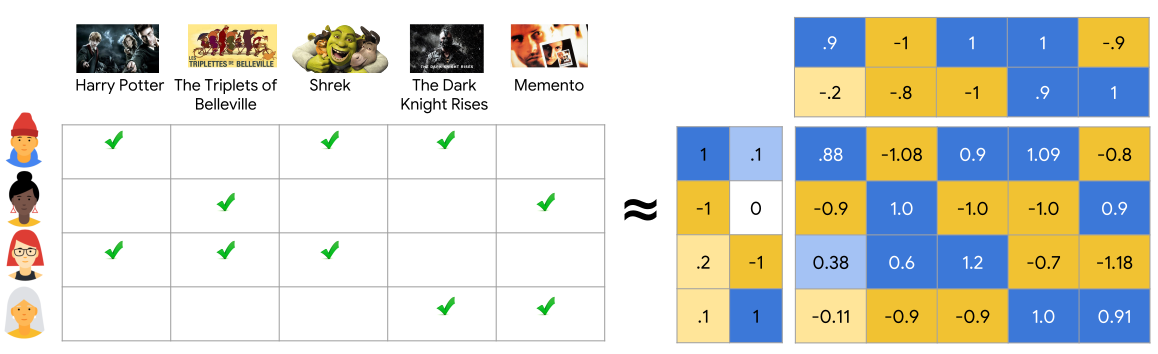
\includegraphics[width=\linewidth]{immagini/matrix_factorization.pdf}
  \caption{Approssimazione matrice dei rating con matrix factorization}
  \cite{mf-google}
  \label{fig:matrix_factorization}
\end{figure}

In \autoref{fig:matrix_factorization} è mostrato come la matrice dei rating $A \in \mathbb{R}^{m \times n}$, con $m$ numero di utenti e $n$ numero di oggetti, viene decomposta in due matrici di dimensionalità molto minore:

\begin{itemize}
	\item Una matrice di fattori latenti per gli utenti $P \in \mathbb{R}^{m \times d}$, in cui la riga $i$ contiene i fattori latenti dell'utente $i$.
	\item Una matrice di fattori latenti per gli oggetti $Q \in \mathbb{R}^{n \times d}$, in cui la riga $j$ contiene i fattori latenti dell'oggetto $j$.
\end{itemize}
Le due matrici di fattori latenti $P$ e $Q$ sono imparate in modo tale che il prodotto $PQ^T$ sia una buona approssimazione della matrice dei rating $A$ \cite{mf-google}. In letteratura esistono diversi algoritmi per calcolare i fattori latenti di utenti e oggetti. Il primo algoritmo proposto è stato FunkSVD \cite{funk-mf} che supporta unicamente feedback espliciti, SVD++ \cite{svd++} aggiunge il bias di utenti e oggetti e il supporto a feedback impliciti; ALS \cite{als} e logistic MF \cite{logistic-mf} sono invece algoritmi progettati con i feedback impliciti in mente.


\subsection{Alternating least square} \label{subsec:als}
Alternating Least Square (ALS) \cite{als} è un algoritmo di matrix factorization stato dell'arte per quanto riguarda i feedback impliciti. ALS è un processo di ottimizzazione iterativo in cui ad ogni iterazione si cerca di arrivare il più vicino possibile a una rappresentazione fattorizzata dei dati originali \cite{als-medium}. 

\subsubsection{Feedback impliciti}
I feedback impliciti sono più semplici da collezionare rispetto ai feedback espliciti. Infatti, mentre i feedback espliciti sono ottenuti da valutazioni che l'utente lascia intenzionalmente sugli oggetti (es. valutazione da 1 a 10 di un film); i feedback impliciti sono collezionati automaticamente osservando il comportamento di un utente (es. 1 se l'utente ha guardato un film, 0 altrimenti).
I feedback impliciti hanno alcune importanti caratteristiche che li distinguono dai feedback espliciti, e impediscono di usare direttamente algoritmi progettati con i feedback espliciti in mente \cite{als}:
\begin{enumerate}
 \item \textit{Non ci sono feedback negativi.} Osservando il comportamento di un utente, è possibile inferire quali oggetti gli interessano e che quindi ha scelto di consumare. \'E difficile però capire in modo affidabile quali oggetti l'utente non apprezza. Per esempio, un utente che non ha guardato una serie tv potrebbe non averlo fatto perchè non interessato a quella serie, oppure perché non la conosceva. Questa asimmetria non esiste nei feedback espliciti in cui un utente si esprime su cosa gli piace e cosa non gli piace. Anche i dati mancanti sono un problema: nei feedback espliciti si conosce quali rating non sono stati espressi dall'utente, nei feedback impliciti no.
 
 \item \textit{I feedback impliciti sono intrinsicamente rumorosi.} Tenendo traccia passivamente dei comportamenti degli utenti è difficile distinguere il caso in cui un utente ha consumato un oggetto perchè davvero interessato o per altri motivi.
 
 \item Il valore numerico dei feedback espliciti indica la \textit{preferenza}, mentre il valore numerico dei feedback impliciti indica la \textit{confidenza}. I sistemi basati sui feedback espliciti permettono all'utente di impostare il loro livello di preferenza su un oggetto, ad esempio con un voto da 1 a 5. I feedback impliciti invece descrivono la frequenza di un'azione, ma un valore più alto  non indica per forza una preferenza maggiore
\end{enumerate}

\subsubsection{Il modello}
Per prima cosa vanno formalizzati i concetti di preferenza e confidenza. La preferenza di un utente $u$ per un item $i$ è indicata con un valore binario $p_{ui}$:
$$
p_{ui} =     \begin{cases}
				1 \;\;\; r_{ui} > 0 \\
				0 \;\;\; r_{ui} = 0
              \end{cases}
$$
In pratica, se un utente $u$ ha consumato un oggetto $i$ ($r_{ui} > 0$), allora si ha un'indicazione che $u$ è interessato a $i$. Diversamente, se $u$ non ha mai consumato $i$ la preferenza è uguale a 0. Inoltre, con l'aumento del valore di $r_{ui}$ si ha un indicazione più forte che l'utente sia davvero interessato all'oggetto. Di conseguenza, si può indicare con $c_{ui}$ la confidenza nell'osservare $p_{ui}$. Una possibile scelta è
$$
c_{ui} = 1 + \alpha r_{ui}
$$
In questo modo, si ha una confidenza minima su $p_{ui}$ per ogni coppia utente-oggetto, ma osservando più preferenze positive la confidenza su $p_{ui} = 1$ aumenta. La velocità di incremento è controllata dalla costante $\alpha$.

Come spiegato nella \autoref{ssec:mf}, l'obiettivo è trovare un vettore $x_u \in R^f$ per ogni utente $u$, ed un vettore $y_i \in R^f$ per ogni oggetto $i$ che fattorizzano le preferenze degli utenti. Le preferenze possono essere poi calcolate come $p_{ui} = x_u^Ty_i$. I vettori latenti in ALS sono calcolati minimizzando la funzione obiettivo:	
$$
\min_{x_*,y_*} \sum_{u,i} c_{ui} (p_{ui} - x_u^Ty_i)^2 + 
\lambda \left( \sum_u ||x_u||^2 + \sum_i ||y_i||^2 \right)
$$
Il termine $\lambda \left( \sum_u ||x_u||^2 + \sum_i ||y_i||^2 \right)$ è necessario per regolarizzare il modello ed evitare l'overfitting durante il training. Il valore esatto di $\lambda$ dipende dai dati e si determina tramite cross validation. 
Quando il vettore latente degli utenti o degli oggetti rimane fissato, la funzione obiettivo diventa quadratica e si può calcolare un minimo globale. Questo porta ad un processo di ottimizzazione con il metodo dei minimi quadrati, in cui si alterna tra il ricalcolare il vettore degli utenti mantenendo fissato quello degli oggetti e viceversa. Ad ogni step il valore della funzione di costo diminuisce.

\subsection{Neural collaborative filtering} \label{subsec:ncf}
Gli algoritmi basati su matrix factorization sono sicuramente i più popolari nell'ambito dei sistemi di raccomandazione collaborative filtering. Nonostante l'efficacia di questi modelli, le loro prestazioni  posso variare in base alla scelta della funzione di interazione. Ad esempio, per quanto riguarda il task di rating prediction su feedback espliciti, è noto che le prestazioni di MF possono essere migliorate incorporando il bias di utenti e oggetti nella funzione di interazione. Anche se si tratta solo di una piccola modifica, dimostra l'effetto positivo di progettare una funzione migliore per modellare l'interazione delle feature latenti di utenti e oggetti. 
Secondo gli autori di \cite{NCF} il prodotto scalare, che combina la moltiplicazione delle feature latenti in modo lineare, potrebbe non essere sufficiente per catturare la complessa struttura dei dati che rappresentano le interazioni dell'utente. 

La \autoref{fig:mf-limits} mostra come il prodotto scalare può limitare l'espressività di MF. La similarità tra due utenti può essere misurata con il prodotto scalare tra i loro vettori latenti, o in modo equivalente con il coseno dell'angolo tra i loro vettori latenti. Dalla matrice utenti-oggetti, in \autoref{fig:mf-limits} indicata con (a), l'utente $u_4$ è più simile a $u_1$, seguito da $u_3$, e in ultimo da $u_2$. Tuttavia, nello spazio latente indicato con (b), posizionare $p_4$ più vicino a $p_1$ rende $p_4$ più vicino a $p_2$ e non a $p_3$.

Viene quindi proposto di usare le reti neurali che sono considerate approssimatori universali \cite{NN-universal-approx} per imparare le interazioni utente-oggetto. In particolare sono proposti tre modelli basati su deep neural network:
\begin{enumerate}
 \item Generalized Matrix Factorization (GMF), illustrato in Sez. \ref{sssec:gmf} 
 \item Multi-Layer Perceptron (MLP), illustrato in Sez. \ref{sssec:mlp} 
 \item Neural Matrix Factorization (NeuMF), , illustrato in Sez. \ref{sssec:neumf} 
\end{enumerate}

\begin{figure}
  \centering
  \includegraphics[scale=0.50]{immagini/user_item_vectors.png}
  \caption{Limitazioni di matrix factorization}
  \cite{NCF}
  \label{fig:mf-limits}
\end{figure}

\subsubsection{Approccio generale}
Per permettere un trattamento neurale di collaborative filtering, viene adottata una rappresentazione multi-layer per modellare le interazioni utente-oggetto $y_{ui}$, in cui l'output di un layer è l'input per il layer successivo. Il layer di input consiste di due vettori $v_u^U$ e $v_i^I$ che descrivono rispettivamente l'utente $u$ e l'oggetto $i$. Dato che l'input nei modelli collaborative filtering è composto dagli ID univoci di $u$ e $i$, essi devono essere convertiti con one-hot encoding in vettori binari sparsi. One-hot encoding è un processo che converte una variabile categorica in un vettore di uno e zero. La lunghezza del vettore in questo caso è pari al numero di utenti o oggetti, ed ogni elemento nel vettore rappresenta un utente/oggetto. Tutti gli elementi del vettore sono posti a zero, tranne l'elemento corrispondente all'utente/oggetto corrente che è posto ad uno. Sopra al layer di input c'è il layer di embedding: è un layer fully connected che proietta la rappresentazione sparsa in un vettore denso. Gli embedding di utenti e oggetti ottenuti possono essere visti come i vettori latenti di utenti e oggetti nel contesto dei modelli a fattori latenti come matrix factorization. I vettori di embedding di user e item sono dati in input a un architettura neurale multi-layer, i cui livelli sono chiamati neural collaborative filtering layer, e infine al layer di output per calcolare lo score predetto $y_{ui}$. Questo approccio generale è chiamato \textit{neural collaborative filtering} (NCF), ed è mostrato in \autoref{fig:ncf}.

\begin{figure}
  \centering
  \includegraphics[width=\linewidth]{immagini/ncf.png}
  \caption{Approccio neural collaborative filtering}
  \cite{NCF}
  \label{fig:ncf}
\end{figure}

\subsubsection{Generalized matrix factorization} \label{sssec:gmf}
In \cite{NCF} viene mostrato come la famiglia di metodi basata su matrix factorization possa essere considerata un caso particolare dell'approccio NCF. Come detto prima, i vettori di embedding possono essere visti come i vettori latenti di utenti e oggetti imparati dagli algoritmi di MF. Siano $p_u$ il vettore latente degli utenti e $q_i$ il vettore latente degli oggetti. Si può ridefinire la funzione del primo neural CF layer per eseguire la moltiplicazione tra i due vettori di embedding:
$$
\phi(p_u, q_1) = p_u \odot q_i
$$
in cui $\odot$ è il prodotto elemento per elemento dei vettori. Si proietta poi il vettore risultato sul layer di output:
$$
y_{ui} = a_{out}(h^T(p_u \odot q_i))
$$
dove $a_{out}$ e $h$ sono rispettivamente la funzione di attivazione e  i pesi del layer di output.  Se si usa una funzione identità per $a_{out}$ e si impone che $h$ sia un vettore uniforme di 1, si può ricostruire esattamente il modello MF. Questo modello è chiamato generalized matrix factorization (GMF).

\subsubsection{Multi-layer perceptron} \label{sssec:mlp}
In questa istanza di NCF, i vettori di embedding di utenti e oggetti ottenuti dai layer di embedding sono concatenati. Sopra al layer di concatenazione sono aggiunti dei layer nascosti, in modo da usare un multi-layer perceptron (MLP) standard per imparare le interazioni tra le feature latenti di utenti e oggetti. In questo caso, il modello impara una funzione non-lineare per le interazioni tra $p_u$ e $q_i$, invece di imparare un prodotto elemento per elemento come GMF. 

\subsubsection{Neural matrix factorization} \label{sssec:neumf}
A questo punto si hanno due diverse implementazioni del framework NCF: GMF che applica un funzione lineare per imparare le interazioni delle feature latenti, e MLP che invece applica un funzione non lineare. Le due reti possono essere combinate per modellare in modo più preciso le complesse interazioni utente-oggetto. Una soluzione semplice è permettere a GMF e MLP di condividere lo stesso layer di embedding; questo approccio però può limitare le performance del modello perchè GMF e MLP devono usare embedding della stessa dimensione. Per fornire più flessibilità al modello fuso, GMF e MLP imparano vettori di embedding separati, e i due modelli sono combinati concatenando l'output del loro ultimo layer nascosto. L'architettura del modello fuso chiamata neural matrix factorization (NeuMF) è mostrata in \autoref{fig:neumf}. A sinistra è rappresentata la rete GMF, a destra il MLP.

\begin{figure}
  \centering
  \includegraphics[width=\linewidth]{immagini/neumf.png}
  \caption{Neural matrix factorization}
  \cite{NCF}
  \label{fig:neumf}
\end{figure}


\subsection{Vantaggi e svantaggi dell'approccio CF} \label{ssec:pros-cons-cf}
\textbf{Vantaggi:}
\begin{itemize}

 \item \textit{Nessuna conoscenza del dominio necessaria:} basandosi solo su interazioni utente - oggetto, il modello può funzionare in domini in cui non c'è nessun contenuto associato agli oggetti \cite{recsys-principle-methods-evaluation}. Questo permette di impiegarlo facilmente per realizzare RS multi-domain, che raccomandano oggetti di natura diversa (audio, film, testo, etc.).
 
 \item \textit{Serendipity:} il modello ha la capacità di fornire consigli fortuiti, il che significa che può consigliare elementi pertinenti per l'utente senza che il contenuto si trovi nel profilo dell'utente, permettendo così all'utente di scoprire nuovi interessi \cite{recsys-principle-methods-evaluation} \cite{cf-advantages-google}.
\end{itemize}

\noindent \textbf{Svantaggi:}
\begin{itemize}
 \item \textit{Problema del cold-start:} si riferisce alla situazione in cui il sistema di raccomandazione non ha abbastanza informazioni su un utente od un oggetto per poter fare previsioni rilevanti. Un nuovo oggetto inserito nel RS di solito non ha voti, ed è quindi improbabile che venga raccomandato. Un oggetto non consigliato passa inosservato a gran parte della community. Il problema è presente anche per i nuovi utenti: gli utenti che hanno espresso nessuna o poche valutazioni non ricevono raccomandazioni affidabili \cite{cold-start}.   
 
 \item  \textit{Problema di data sparsity:} questo è il problema che si verifica a causa della mancanza di informazioni sufficienti, cioè quando solo pochi rispetto al numero totale di oggetti disponibili in un database sono valutati dagli utenti. Ciò porta ad una rating matrix sparsa, e raccomandazioni poco efficaci \cite{recsys-principle-methods-evaluation}.
 
 \item \textit{Scalabilità:} questo è un altro problema associato agli algoritmi di raccomandazione perché il tempo di computazione cresce linearmente sia con il numero di utenti, sia con il numero di oggetti. Un sistema di raccomandazione efficiente con un dataset limitato potrebbe non esserlo con un dataset di dimensioni maggiori \cite{recsys-principle-methods-evaluation}.
\end{itemize}


\section{Content-based recommender system}
Nei recommender system content-based (CB), gli attributi descrittivi degli oggetti sono usati per produrre raccomandazioni. Il termine ``content" indica che il processo di raccomandazione si focalizza sui contenuti piuttosto che sulle interazioni utente - oggetto. Nei metodi content-based i rating degli utenti sono combinati con le informazioni disponibili sugli oggetti, per poi essere usati come training data per creare un modello di classificazione o regressione  specifico per l'utente. Nei problemi di classificazione si prevede se ad un utente può piacere un oggetto; nei problemi di regressione si prevede il rating dato da un utente ad un oggetto la cui valutazione è ancora sconosciuta \cite{recsys-book}.

Mentre nei CF la similarità tra due oggetti (o due utenti) è calcolata come la correlazione o la similarità tra i rating forniti dagli altri utenti, i recommender system content-based sono progettati per consigliare oggetti simili a quelli che l'utente ha preferito in passato. Non considerando gli altri utenti, la lista di raccomandazioni può essere generata anche se c'è un solo utente nel sistema.

\subsection{Vantaggi e svantaggi dell'approccio CB}
\textbf{Vantaggi:}
\begin{itemize}
 \item \textit{Consigliare nuovi oggetti:} questi modelli hanno la capacità di consigliare nuovi oggetti anche se non ci sono valutazioni fornite dagli utenti, a differenza dei modelli collaborative filtering \cite{recsys-principle-methods-evaluation}.
 
 \item \textit{Trasparenza:} le spiegazioni su come funziona il sistema di raccomandazione possono essere fornite elencando esplicitamente le caratteristiche del contenuto che hanno causato la presenza di un oggetto nell'elenco delle raccomandazioni \cite{transparency}. 
\end{itemize}

\noindent \textbf{Svantaggi:}
\begin{itemize}
 \item \textit{Feature degli oggetti:} la precisione del modello dipende dall'insieme delle feature che descrivono gli oggetti. Identificare le feature più rilevanti non è semplice e dipende molto dall'applicazione specifica \cite{survey-mattia}.
 
 \item \textit{Content overspecialization:} dato che i metodi CB si affidano solo alle caratteristiche degli oggetti già valutati dall'utente corrente, egli riceverà solo raccomandazioni simili ad altri oggetti già definiti nel suo profilo \cite{recsys-principle-methods-evaluation}.
 
 \item \textit{Raccomandazioni multi-dominio:} è difficile creare RS multi-dominio con un approccio content-based. Questo perché è complicato definire un insieme di feature che valgano per contenuti di natura diversa.
\end{itemize}

\section{Hybrid recommender system}
I modelli ibridi combinano tipi diversi di sistemi di raccomandazione per formare dei modelli in grado di superare le debolezze dei modelli singoli. In \cite{recsys-book} sono descritti tre modi per creare recommender system ibridi:

\begin{enumerate}
 \item \textit{Ensemble design:} Con questo metodo i risultati degli algoritmi base sono combinati in un output singolo più robusto. Il principio fondamentale è molto simile ai metodi di ensemble usati in molte applicazioni di data mining come clustering, classificazione e analisi degli outlier. 
Gli ensemble design possono essere formalizzati nel modo seguente. Sia $R^k$ una matrice $m \times n$ contenente le predizioni di $m$ utenti per $n$ oggetti dell'algoritmo $k$-esimo, con $k \in \{1, \dots ,q\}$. Pertanto, un totale di $q$ algoritmi diversi sono usati per ottenere queste predizioni. L'elemento $(u,j)$-esimo di $R^k$ contiene il rating predetto per l'utente $u$ sull'oggetto $j$ dall'algoritmo $k$-esimo. Gli elementi della matrice originale $R$ sono replicati in ogni $R^k$, e solo gli elementi non presenti in $R$ variano nei differenti $R^k$ a causa dei diversi risultati degli algoritmi. Il risultato finale è ottenuto combinando le predizioni $R^1, \dots, R^q$ in un singolo output. La combinazione può essere fatta in vari modi, ad esempio calcolando la media pesata delle varie predizioni. Le caratteristiche comuni di questi algoritmi sono: (i) usare sistemi di raccomandazione già esistenti, (ii) produrre uno score/ranking unico. Il problema di questo approccio è la complessità della soluzione: il risultato è ottenuto con l'esecuzione di $q$ algoritmi di raccomandazione diversi.

 \item \textit{Monolithic design:} In questo caso, viene creato un algoritmo di raccomandazione integrato utilizzando vari tipi di dati. A volte non esiste una chiara distinzione tra le varie parti (es. content-based e collaborative filtering) dell'algoritmo. In altri casi, potrebbe essere necessario modificare algoritmi di raccomandazione esistenti per essere usati all'interno dell'approccio generale, anche quando c'è una chiara distinzione tra gli algoritmi utilizzati.  Pertanto, questo metodo tende a integrare più strettamente le varie fonti di dati e non è possibile visualizzare facilmente i singoli componenti come black-box separate.
 
 \item \textit{Mixed system:}  Come per gli ensemble, questi sistemi usano diversi algoritmi di raccomandazione come black-box, ma gli oggetti raccomandati dai vari sistemi sono presentati insieme senza essere combinati.
\end{enumerate} 

\section{Context-aware recommender system}
La maggior parte degli approcci esistenti per sviluppare sistemi di raccomandazione si concentra sul raccomandare gli oggetti più rilevanti ai singoli utenti senza considerare informazioni aggiuntive come il tempo, il luogo, etc. In altre parole, i sistemi di raccomandazione tradizionalmente si occupano di applicazioni che hanno solo due tipi di entità, utenti ed oggetti, e non li inseriscono in un contesto quando forniscono raccomandazioni. Tuttavia, in molte applicazioni potrebbe non essere sufficiente considerare solo utenti ed oggetti, ma è anche importante incorporare informazioni contestuali nel processo di raccomandazione al fine di consigliare oggetti agli utenti in determinate circostanze. I sistemi di raccomandazione che producono le loro raccomandazioni utilizzando il contesto sono chiamati recommender system context-aware (CARS). Alcuni esempi di contesto sono:

\begin{enumerate}
 \item \textit{Data e ora:} Dalle informazioni di data e ora è possibile estrarre diverse feature contestuali come il momento della giornata, il giorno della settimana, week-end, vacanze, stagioni ed altro ancora. Una raccomandazione potrebbe essere rilevante la mattina ma non il pomeriggio, e viceversa. Le raccomandazioni sui vestiti invernali o estivi possono essere molto diverse.
 \item \textit{Posizione:} Con la crescente popolarità del GPS disponibile ormai su qualunque telefono, le raccomandazioni sensibili alla posizione dell'utente hanno guadagnato importanza. Per esempio, un viaggiatore potrebbe desiderare raccomandazioni su ristoranti vicini alla propria posizione. Questo può essere fatto aggiungendo la posizione come contesto nel recommender system.
 \item \textit{Informazioni sociali:} Il contesto sociale è spesso importante per un sistema di raccomandazione. Le informazioni su amici, tag e relazioni sociali di un utente possono avere un impatto sul processo di raccomandazione. Per esempio un ragazzo potrebbe scegliere di guardare un film diverso a seconda che lo guardi con i suoi genitori o con i suoi amici.
\end{enumerate} 

% aggiungere esempi di CARS in letteratura

\noindent Il contesto può essere ottenuto in vari modi \cite{recsys-handbook} che includono:
\begin{enumerate}
 \item \textit{Esplicitamente} ponendo domande dirette alle persone rilevanti o richiedendo le informazioni con altri mezzi. Per esempio, un sito web potrebbe ottenere informazioni contestuali chiedendo agli utenti di compilare un form.
 \item \textit{Implicitamente} dai dati o dall'ambiente, come il cambio di posizione rilevato da una compagnia di telefonia mobile. In questo caso non è necessario fare nulla in termini di interazione con l'utente perché l'informazione contestuale è acceduta direttamente e i dati sono estratti da essa.
 \item \textit{Per inferenza} usando metodi statistici o di data mining. 
\end{enumerate}
In letteratura sono stati proposti diversi sistemi di raccomandazione che integrano informazioni contestuali: in \cite{mf-context-aware} vengono ideati tre diversi metodi per consentire a MF di supportare informazioni di contesto, in \cite{tensor-context-aware} viene proposto un modello di tensor factorization context aware, in \cite{context-aware-deep-learning} è usato un approccio deep-learning per produrre raccomandazioni context-aware con una rete neurale. Per quanto riguarda le raccomandazioni in ambito mobile, in \cite{cars-music2} viene usato il contesto corrente dell'utente e i suoi ascolti passati per generare una playlist di canzoni. In \cite{cars-music} viene usato il contesto raccolto da uno smart device per raccomandazioni musicali, in \cite{cars-location} viene sfruttata la posizione dell'utente per fornire raccomandazioni su luoghi o eventi nelle vicinanze. Tutti questi sistemi producono raccomandazioni context-aware per dispositivi mobili, ma il RS non è implementato direttamente sul dispositivo dell'utente.

\subsection{Approccio multidimensionale} \label{subsec:multidim}
Il problema tradizionale di raccomandazione può essere visto come l'apprendimento di una funzione che associa le coppie utente-oggetto ai rating. La funzione corrispondente $f_R$ è definita come:

$$
f_R : U \times I \rightarrow rating
$$
Quindi la rating function mappa da uno spazio bidimensionale di utenti e oggetti ai rating.
I CARS generalizzano questo metodo utilizzando un approccio multidimensionale in cui la rating function può essere vista come un mapping da una matrice $n$-dimensionale all'insieme dei rating \cite{survey-mattia}.
$$
f_R : D_1 \times D_2 \dots \times D_n \rightarrow rating
$$
In questo caso, il risultato è un cubo n-dimensionale invece di una matrice bidimensionale. Le diverse dimensioni sono denotate come $D_1 \dots D_n$. Due di queste dimensioni saranno sempre utenti e oggetti, le altre $D_i$ dimensioni corrispondono alle feature del contesto \cite{recsys-book}. In \autoref{fig:ratings-cube} è mostrato un esempio di un cubo tridimensionale che memorizza i ratings per $User \times Item \times Location$, in cui $f_R(u_1, i_4, home) = 5$ significa che l'utente $u_1$ ha valutato con un punteggio pari a 5 l'oggetto $i_4$ mentre era a casa.

Il contesto può essere applicato nelle varie fasi del processo di raccomandazione. Come rappresentato in \autoref{fig:context-paradigm} si possono identificare tre paradigmi principali per integrare il contesto nei sistemi di raccomandazione \cite{recsys-handbook}:

\begin{figure}
  \centering
  \includegraphics[scale=0.75]{immagini/rating_cube.png}
  \caption{Esempio di un cubo multidimensionale per $User \times Item \times Location$}
  \cite{survey-mattia}
  \label{fig:ratings-cube}
\end{figure}

\begin{enumerate}
 \item \textit{Contextual pre-filtering:} In questo paradigma, le informazioni riguardo il contesto attuale sono utilizzate per selezionare o costruire l'insieme dei dati rilevanti (la matrice dei rating). Poi i rating mancanti dai dati selezionati possono essere predetti utilizzando qualsiasi sistema di raccomandazione 2D tradizionale.
 \item \textit{Contextual post-filtering:} In questo paradigma, le informazioni contestuali sono inizialmente ignorate e i rating sono predetti utilizzando qualsiasi sistema di raccomandazione 2D tradizionale. Poi, l'insieme di raccomandazioni non rilevanti nel contesto $c$ sono filtrate, e la lista di raccomandazioni è regolata in base a $c$.
 \item  \textit{Contextual modeling:} Mentre gli approcci di contextual pre-filtering e post filtering fanno uso di una funzione di raccomandazione 2D, gli approcci di contextual modeling danno luogo a funzioni di raccomandazione veramente multidimensionali che rappresentano modelli predittivi o euristiche che incorporano informazioni contestuali in aggiunta ai dati di utenti e oggetti.
\end{enumerate}

\begin{figure}
  \centering
  \includegraphics[width=\linewidth]{immagini/paradigm_for_context_inclusion.png}
  \caption{Paradigmi per incorporare il contesto nei sistemi di raccomandazione}
  \cite{context-paradigm}
  \label{fig:context-paradigm}
\end{figure}

%spostare in context aware
\subsection{Raccomandazioni context-aware con modelli di deep learning}
I sistemi di raccomandazione context-aware tradizionali come matrix factorization \cite{mf-context-aware} o tensor factorization \cite{tensor-context-aware}, usano principalmente un insieme selezionato di informazioni contestuali. Il contesto specifico descrive le circostanze in cui le informazioni sono state raccolte, quali ad esempio il meteo (soleggiato, nuvoloso, etc.), o il tempo (giorno della settimana, ora, etc.). Il vantaggio principale è la bassa dimensionalità del contesto che permette di integrarlo facilmente nei sistemi di raccomandazione esistenti \cite{context-aware-deep-learning}. Infatti un dataset con molte feature porta naturalmente ad uno spazio multidimensionale e quindi a sparsità.

Tuttavia, i CARS tradizionali  hanno le seguenti limitazioni: (1) la selezione del contesto specifico è un task che richiede tempo essendo fatto a mano da esperti di dominio, (2) il contesto selezionato potrebbe non rappresentare l'insieme di feature contestuali più efficace per il recommender system in questione; (3) l'utilizzo di contesti espliciti, come la posizione dell'utente, può sollevare problemi di privacy  \cite{context-aware-deep-learning}. La limitazione sul numero di feature contestuali potrebbe essere un problema in quegli ambienti in cui il contesto è complesso e dinamico. Ad esempio, sfruttando i numerosi sensori presenti sugli smartphone come accelerometro, campo magnetico, GPS, e sensore di luminosità, possono essere raccolte informazioni di contesto ad alta dimensionalità. Queste informazioni sono poi utilizzate per inferire il contesto e il comportamento dell'utente; dall'accelerometro si può capire l'attività dell'utente (es. camminare, stare seduto, correre), mentre con il GPS si può inferire la posizione (es. a casa, al lavoro, all'aperto).

Per risolvere i problemi legati all'utilizzo del contesto multidimensionale, viene proposto in letteratura di ridurre la dimensionalità del contesto con autoencoder o Principal Component Analysis (PCA) \cite{latent-context} \cite{context-autoencoder}, di costruire una rappresentazione gerarchica del contesto \cite{hierarchical-context}, e di usare dei modelli di deep learning in grado di supportare molte feature di contesto\cite{context-aware-deep-learning}.

\subsubsection{Estrazione del contesto latente} 
\label{ssec:latent-context}
\begin{figure}
 \centering
  \includegraphics[scale=0.50]{immagini/autoencoder.png}
  \caption{Esempio struttura di un autoencoder}
  \cite{hierarchical-context}
  \label{fig:ae}
\end{figure}

Come detto prima, il contesto ad alta dimensionalità è spesso composto da dati di sensori (GPS, accelerometro, etc.) che possono essere correlati tra loro. Si può usare un autoencoder (AE) per scoprire le correlazioni tra feature differenti ed estrarre una rappresentazione a bassa dimensionalità del contesto \cite{latent-context}. Un autoencoder è una rete neurale che trasforma l'input ad alta dimensionalità in una rappresentazione latente a bassa dimensionalità (encoder), poi esegue una ricostruzione dell'input originale a partire dalla rappresentazione latente (decoder) \cite{autoencoder}. Limitando il numero di unità nei layer nascosti di un AE, la rete è costretta a imparare una rappresentazione compressa dell'input. In \autoref{fig:ae} è rappresentata la struttura di un autoencoder che ricostruisce il vettore di contesto dato in input $\overrightarrow{Context_t}$. Il contesto ottenuto può essere usato al posto delle feature di contesto estratte dai dati raw, e può portare ad un miglioramento nelle raccomandazioni prodotte dal recommender system.

L'algoritmo \autoref{alg:latent-context} descrive come utilizzare un AE per estrarre gli attributi latenti del contesto. L'input per l'algoritmo è un training set $S = \{s_1, s_2, \dots, s_n\}$, in cui ogni campione è $r-$dimensionale e contiene le feature di contesto estratte dai dati raw, $f$ è la funzione di attivazione dell'autoencoder. L'output è $O$, l'insieme delle feature latenti estratte da $S$. L'algoritmo inizia normalizzando il dataset $S$ (riga 1); la normalizzazione include la conversione delle variabili categoriche in valori binari e la normalizzazione delle variabili numeriche. Il risultato è il dataset normalizzato $S'$. Poi viene eseguito il training di un AE sul training set normalizzato (riga 2). A training terminato si ricava la matrice $W$, in cui $w_{ij}$ è il peso dell'arco che connette il neurone di input $j$-esimo con il neurone nascosto $i$-esimo (riga 3). Dopo aver inizializzato $O$ (riga 4), si itera su ogni sample di $S'$ (riga 5), moltiplicandolo per la trasposta di $W$ (riga 6), e applicando la funzione di attivazione $f$ su ogni elemento del vettore risultato (riga 7). Questo vettore è concatenato a $O$ che a ciclo terminato viene ritornato (riga 9). Le righe 10, 11 e 12 descrivono come estrarre il contesto latente da un nuovo campione $t$. Per prima cosa $t$ viene normalizzato esattamente come nella riga 1, poi usando la matrice $W$ e la funzione di attivazione $f$ si ottiene il contesto latente $res$.

\begin{algorithm}
\floatname{algorithm}{Algoritmo}
\caption{Estrarre il contesto latente usando un auto-encoder \cite{latent-context}}
\label{alg:latent-context}
 \hspace*{\algorithmicindent} \textbf{Input:} $S$ - training set, $n$ latent context size, $f$ - activation function.\\
 \hspace*{\algorithmicindent} \textbf{Output:} $O$ - latent context attributes of the training set; extraction function\\ 
 \hspace*{\algorithmicindent} for a new sample $t$
\begin{algorithmic}[1]
\STATE $S' \leftarrow$ Normalize all samples in $S$
\STATE $AE \leftarrow$ Train an auto-encoder $(n,f)$ on the normalized training dataset $S'$
\STATE $W \leftarrow$ Retrieve weight matrix from $AE$
\STATE $O \leftarrow \varnothing$
\FORALL{$s' \in S'$} 
	\STATE $o \leftarrow s'W^T$
	\STATE $O \leftarrow O \; \cup$ activate $f$ on each element in $o$ 
\ENDFOR

\STATE Return $O$

Extraction for a new data sample $t$:
\STATE $t' \leftarrow$ normalize $t$
\STATE $res \leftarrow$ activate $f$ on each element in $t'W^T$ 
\RETURN $res$

\end{algorithmic}
\end{algorithm}


Nonostante la rappresentazione compressa del contesto possa portare a delle raccomandazioni più precise, l'applicazione di questa tecnica non è consigliabile in ambiente mobile. Il problema in ambiente mobile è che il dataset $S$ è in continua evoluzione, e nuovi campioni $t$ sono aggiunti al dataset quando un utente interagisce con altri dispositivi tramite comunicazione D2D. Questo significa che il contesto latente calcolato con la matrice $W$ ottenuta dall'autoencoder con training sul dataset $S$, dovrà essere aggiornato nel momento in cui sono ottenuti nuovi campioni $t$ di contesto. Aggiornare il contesto latente significa continuare il training dell'autoencoder sull'insieme dei nuovi campioni $S^1$, ricavare la matrice $W$ dei pesi a training finito, e calcolare il contesto latente per i campioni vecchi e nuovi. Questo processo aggiunge una complessità indesiderabile che non giustifica il miglioramento nelle prestazioni del RS.

\subsubsection{Rappresentazione gerarchica del contesto}
\label{ssec:hierarchical}
Il metodo per ridurre la dimensionalità del contesto descritto nella \autoref{ssec:latent-context} modella le informazioni contestuali in vettori a dimensionalità minore, ignorando però la struttura delle variabili latenti di contesto. In particolare, questi metodi, mentre riducono la dimensionalità dello spazio contestuale, non tengono conto della struttura delle variabili latenti di contesto e delle relazioni semantiche tra queste variabili. In \cite{hierarchical-context} viene proposta una nuova rappresentazione strutturata del contesto latente organizzata in maniera gerarchica che include gruppi di contesti latenti simili chiamati \textit{situazioni contestuali}. Per esempio, se un vettore latente del contesto rappresenta le variabili di contesto ``mattina", ``rumoroso", ``fermo" e la posizione è ``università", allora queste variabili di contesto collettivamente rappresentano la situazione di uno studente che segue una lezione in università. Le situazioni contestuali possono poi essere organizzate in una struttura gerarchica aggregando i vettori latenti del contesto in una rappresentazione ad alto livello. Per esempio, ``seguire una lezione in università" e ``pranzare in università" possono essere aggregati in una situazione contestuale più ad alto livello come ``essere situati in università".

\begin{figure}
 \centering
  \includegraphics[scale=0.70]{immagini/hierarchical.png}
  \caption{Gerarchia delle situazioni contestuali}
  \label{fig:hierarchical}
  \cite{hierarchical-context}
\end{figure}

Il processo di costruzione del modello gerarchico è svolto raggruppando l'insieme di tutti i vettori latenti non strutturati del contesto in un insieme finito di cluster, in cui ogni cluster rappresenta una situazione contestuale. Si applica Agglomerative Hierarchical Clustering (AHC) \cite{AHC} ai vettori latenti per stimare in automatico il numero di situazioni contestuali $S$ che sono rappresentate come cluster. Poi si applica l'algoritmo k-means  per raggruppare vettori simili nella stessa situazione contestuale. Il clustering gerarchico produrrà un albero come quello in \autoref{fig:hierarchical}. Per ogni vettore del contesto latente $\overrightarrow{lc_j}$, i quali sono sempre nodi foglia dell'albero, esiste un nodo $s_{h_ti}$ che è un antenato del nodo $\overrightarrow{lc_j}$. Il nodo $s_{h_ti}$ rappresenta una situazione contestuale simile per il vettore $\overrightarrow{lc_j}$ al livello $h_t$ della gerarchia. Il contesto gerarchico per un vettore $\overrightarrow{lc_j}$ è il percorso dalla sua foglia fino alla radice dell'albero. Per esempio il contesto gerarchico per il vettore di contesto latente $\overrightarrow{lc_{19}}$ in \autoref{fig:hierarchical}, è $\overrightarrow{hlc_{19}} = [s_{19}, s_{26}, s_{33}, s_{41}]$.

L'estrazione del contesto gerarchico è un'operazione irrealizzabile su dispositivo mobile. Infatti, come è sottolineato in \cite{hierarchical-context}, il training di un autoencoder su $n$ vettori di contesto per comprimere le feature di contesto originali da $l$ a $r$ dimensioni, ha una complessità di $O(n \cdot l \cdot r)$. Per estrarre il contesto gerarchico dai vettori di contesto latente viene applicato AHC che ha complessità $O(n^2)$ per $n$ osservazioni. AHC richiede inoltre $O(n^2)$ memoria, che è un requisito troppo alto per dispositivi mobili. 

\subsubsection{Modelli CARS deep learning}
In \cite{context-aware-deep-learning} viene proposto di estendere il modello NeuMF \cite{NCF} descritto nella \autoref{subsec:ncf} aggiungendo un nuovo componente di informazioni contestuali: un vettore di contesto denotato come "Context ($c$)". Il vettore del contesto $c$ è concatenato ai vettori di embedding degli utenti $u$ e degli oggetti $i$ per imparare una nuova funzione tra i tre componenti (utenti, oggetti, e contesto). In questo modo, la dimensione del contesto viene considerata all'interno del framework neurale e la rete apprende automaticamente la sua influenza sul valore di output. Il contesto è concatenato solo agli embedding del multi-layer perceptron, mentre la parte della rete denominata come generalized matrix factorization e i suoi embedding rimangono invariati. \`E importante notare che il vettore di contesto può avere un'alta dimensionalità, infatti questo modello non soffre del problema di ``curse of dimensionality" che affligge i CARS tradizionali.
\begin{figure}
  \centering
  \includegraphics[width=\linewidth]{immagini/cars-ncf.png}
  \caption{Estensione di NeuMF con features di contesto}
  \label{fig:context-neumf}
  \cite{context-aware-deep-learning}
\end{figure}

Le informazioni contestuali sono modellate come un insieme di feature di contesto esplicite, latenti non strutturate o latenti strutturate (gerarchiche). Questo dà luogo a tre diverse estensioni di NeuMF:
\begin{enumerate}
 \item \textit{Explicit context-aware model (ECAM)}: tutto il contesto disponibile viene incorporato nel modello.
 \item \textit{Unstructured context-aware model (UCAM)}: il contesto viene processato da un autoencoder \cite{latent-context} come descritto nella \autoref{ssec:latent-context} prima di essere incorporato nel modello.
 \item \textit{Hierarchical context-aware model (HCAM)}: il contesto viene organizzato in un albero gerarchico \cite{hierarchical-context} come descritto nella \autoref{ssec:hierarchical} prima di essere incorporato nel modello.
\end{enumerate}
In \autoref{fig:context-neumf} è schematizzato il modello NeuMF  esteso per supportare il vettore del contesto. A sinistra è rappresentata la rete GMF, a destra il MLP con il vettore del contesto.


\section{Problemi RS client-server} \label{sec:trad-rs-prob}
% rimuovere le ripetizioni, seguire correzioni prof
In letteratura la stragrande maggioranza dei RS proposti si basa su un'architettura client-server. Il RS che esegue sul server ha una conoscenza completa di utenti, oggetti e rating. Il client, fisso o mobile, esegue delle query al RS per ricevere raccomandazioni. I problemi nel realizzare un RS context-aware che esegue sul dispositivo locale dell'utente sono principalmente due:
\begin{enumerate}
 \item I sistemi di raccomandazione mobile hanno una conoscenza solo parziale di utenti, oggetti, e dei feedback che gli utenti hanno lasciato sugli oggetti. Questo è dovuto al fatto che il RS inizialmente è a conoscenza solo dei feedback dell'utente locale, e ne scopre di nuovi tramite comunicazione D2D con altri dispositivi. 
 
 \item \`E difficile integrare le numerose informazioni di contesto fisico generate dai dispositivi mobili, e le informazioni di contesto sociale che caratterizzano la situazione dell'utente.
\end{enumerate}
Più nel dettaglio per gli algoritmi visti in questo capitolo:


\myparagraph{ALS}
L'input di ALS (\autoref{subsec:als}) è una matrice $R$ di dimensione $u \times i$ con $u$ numero di utenti, e $i$ numero di oggetti. In ambiente mobile inizialmente la matrice $R$ è vuota perché l'utente non ha espresso nessuna valutazione e non ha incontrato altri utenti. Ogni volta che un nuovo utente o un nuovo oggetto viene scoperto, si aggiunge una nuova riga/colonna alla matrice $R$. Il primo problema di questo algoritmo, e più in generale degli algoritmi di matrix factorization, è l'aggiunta di un nuovo utente/oggetto che comporta un cambiamento nella dimensione della matrice $R$. \textit{L'algoritmo deve essere addestrato nuovamente da zero} sulla nuova matrice $R$ per poter raccomandare i nuovi oggetti, e tenere conto delle valutazioni dei nuovi utenti. Il secondo problema di MF è l'aggiunta del contesto. Come detto nella \autoref{subsec:multidim}, ogni feature di contesto è una dimensione aggiunta alla matrice dei rating $R$. Per mantenere una complessità computazionale bassa, per i modelli MF context-aware si seleziona un insieme molti limitato di feature contestuali, che potrebbero non rappresentare pienamente il contesto corrente dell'utente.

\myparagraph{NeuMF}
Neural matrix factorization (\autoref{subsec:ncf}) implementa un RS
collaborative-filtering con una deep neural network. La dimensione dell'input della rete, e di conseguenza la dimensione dell'input del layer di embedding è da definire a livello di compilazione della rete prima di eseguire il training. Una volta terminato il training, la rete è in grado di predire i rating solo degli stessi utenti/oggetti già presenti durante il training. Questo perché l'input deve avere la  dimensione definita a livello di compilazione, e di conseguenza il numero di utenti e oggetti è lo stesso definito a livello di compilazione. Come per ALS, aggiungere un nuovo utente od un nuovo oggetto significa dover compilare di nuovo il modello ed eseguire il training da zero. Questo modello inoltre, come presentato in \cite{NCF} non ha nessun supporto per le feature di contesto.

\myparagraph{Context-aware NeuMF}
Context-aware neural matrix factorization è un estensione di NeuMF che supporta le feature di contesto. Rimangono le stesse limitazioni di NeuMF sull'input, dato che gli ID di utenti e oggetti sono dati in input come vettori in one-hot encoding con dimensione fissata.
